\chapter{Αποτελέσματα Αξιολόγησης σε Spike}
\label{ch:results}

Στα~\cref{ch:polymul-optimization,ch:kernel-optimization} παρουσιάστηκαν
οι βελτιστοποιήσεις τριών υπολογιστικών πυρήνων: πολυωνυμικού πολλαπλασιασμού,
Keccak και αποκωδικοποίησης, σε τρεις βαθμίδες (Tier~1–3). Το παρόν
κεφάλαιο ποσοτικοποιεί τα αποτελέσματα αυτών των βελτιστοποιήσεων μέσω
συστηματικών μετρήσεων \instret στο Spike \gls{iss} (VLEN $= \num{256}$~bits),
ξεκινώντας από απομονωμένα microbenchmarks ανά πυρήνα και καταλήγοντας
στην αξιολόγηση του πλήρους \gls{kem} μέσω των τριών λειτουργιών του (\KeyGen, \Encaps, \Decaps).

\section{Απομονωμένα microbenchmarks}
\label{sec:microbenchmarks}

Η απομονωμένη μέτρηση κάθε πυρήνα εξαλείφει τις αλληλεπιδράσεις μεταξύ
υποσυστημάτων και αποκαλύπτει την καθαρή αλγοριθμική βελτίωση ανά tier.
Κάθε microbenchmark εκτελεί ακριβώς μία κλήση της αντίστοιχης συνάρτησης. 
Το~\cref{fig:microbench-bar} παρουσιάζει συγκεντρωτικά τη σύγκριση
reference–optimized για τους τρεις πυρήνες στο HQC-128 ανά Tier, ενώ οι επιμέρους
πίνακες που ακολουθούν αναλύουν τα αποτελέσματα ανά security level.

\begin{figure}[htbp]
  \centering
  % Grouped bar chart: micro-benchmark instret comparison (HQC-128)
% Shows Reference vs Tier 1/2/3 for each kernel
\tikzsetnextfilename{ch8-results-microbench-bar-chart}
\begin{tikzpicture}
\begin{axis}[
    ybar,
    bar width=10pt,
    width=0.95\textwidth,
    height=7cm,
    ymode=log,
    log origin=infty,
    ylabel={Δυναμικές εντολές (\instret)},
    symbolic x coords={Polymul, Keccak, Decode},
    xtick=data,
    x tick label style={font=\small},
    ymin=10000,
    ymax=100000000,
    legend style={
      at={(0.5,1.03)},
      anchor=south,
      legend columns=3,
      font=\footnotesize,
      /tikz/every even column/.append style={column sep=8pt}
    },
    nodes near coords style={font=\tiny, rotate=90, anchor=west},
    enlarge x limits=0.25,
    grid=major,
    ymajorgrids=true,
    xmajorgrids=false,
]

% Reference (scalar baseline)
\addplot[fill=gray!60, draw=gray!80] coordinates {
    (Polymul, 18504302)
    (Keccak, 758580)
    (Decode, 1052692)
};

% Tier 1 (scalar_zb polymul / opt keccak / scalar-zb decode)
\addplot[fill=blue!50, draw=blue!70] coordinates {
    (Polymul, 182726)
    (Keccak, 554900)
    (Decode, 604218)
};

% Tier 2 (vector_rvv polymul / opt keccak / rvv decode)
\addplot[fill=orange!60, draw=orange!80] coordinates {
    (Polymul, 148479)
    (Keccak, 554900)
    (Decode, 134737)
};

% Tier 3 (vector_zvk polymul / zvbb keccak / zvbc decode)
\addplot[fill=green!50, draw=green!70] coordinates {
    (Polymul, 70070)
    (Keccak, 554900)
    (Decode, 73769)
};

\legend{Reference, Tier~1 (\Zbc), Tier~2 (RVV), Tier~3 (\Zvbc/\Zvbb)}

\end{axis}
\end{tikzpicture}

  \caption{Σύγκριση \instret ανά πυρήνα και tier για HQC-128 (λογαριθμική
    κλίμακα).}
  \label{fig:microbench-bar}
\end{figure}

%% --------------------------------------------------------------------------
\paragraph{Πολυωνυμικός πολλαπλασιασμός.}
Και τα τρία tiers επιταχύνουν τον πολυωνυμικό πολλαπλασιασμό σε όλα τα security
levels, με το μεγαλύτερο κέρδος στο Tier~3:

\begin{table}[htbp]
  \centering
  \caption{Isolated polymul \instret ανά tier και ανά security level (Spike, VLEN $= \num{256}$).}
  \label{tab:microbench-polymul}
  % Table: Polymul micro-benchmark results (all tiers, all security levels)
% All speedups computed vs scalar_ref baseline
\begin{tabular}{l l S[table-format=9.0] S[table-format=6.0] S[table-format=3.1]}
  \toprule
  \textbf{Security Level} & \textbf{Variant} & {\textbf{\instret}} & {\textbf{Code size (B)}} & {\textbf{Speedup}} \\
  \midrule
  \multirow{4}{*}{HQC-128}
    & \code{scalar\_ref}     & 18639752 &  2292 & {—} \\
    & \code{scalar\_zb}  &   186629 & 15270 & {99.9} \\
    & \code{vector\_rvv}  &   140487 &  7992 & {132.7} \\
    & \code{vector\_zvk} &    63804 &  5830 & {292.1} \\
  \midrule
  \multirow{4}{*}{HQC-192}
    & \code{scalar\_ref}     & 56702057 &  2316 & {—} \\
    & \code{scalar\_zb}  &   591557 & 17258 & {95.9} \\
    & \code{vector\_rvv}  &   439516 & 10560 & {129.0} \\
    & \code{vector\_zvk} &   189388 &  8034 & {299.4} \\
  \midrule
  \multirow{4}{*}{HQC-256}
    & \code{scalar\_ref}     & 139877019 & 2314 & {—} \\
    & \code{scalar\_zb}  &  1306068 & 15090 & {107.1} \\
    & \code{vector\_rvv}  &   1014499 & 7648 & {137.9} \\
    & \code{vector\_zvk} &    272896 & 7274 & {512.6} \\
  \bottomrule
\end{tabular}

\end{table}

Παρατηρούμε ότι η βελτιστοποιημένη υλοποίηση κλιμακώνεται με το $N$
αποδοτικότερα από το reference. Και οι δύο υλοποιήσεις χρησιμοποιούν
Karatsuba, όμως το reference καταλήγει σε bit-serial schoolbook στα φύλλα, 
το οποίο κυριαρχεί χρονικά (\pct{96} των
εντολών): το κόστος αυξάνεται $\num{18504302} \to \num{139222953}$
(\num{7.52}$\times$) με πρακτικό εκθέτη $p = \log(\num{7.52}) / \log(\num{57637}/\num{17669}) \approx 1.7$, δηλαδή χειρότερα από τη
θεωρητική κλιμάκωση Karatsuba ($\log_2 3 \approx 1.59$). Το Tier~3
αντικαθιστά τα schoolbook φύλλα με hardware \insn{vclmul} και εκτελεί διανυσματικά τη XOR ανασύνθεση
του Karatsuba. Σε αυτό το εύρος μεγεθών το σταθερό overhead της διανυσματοποίησης 
αποσβένεται όσο μεγαλώνει το $N$, οπότε το κόστος αυξάνεται μόνο
$\num{70070} \to \num{318972}$ (\num{4.55}$\times$), με πρακτικό εκθέτη
$\sim 1.29$, δηλαδή καλύτερη κλιμάκωση από Karatsuba. Αυτή η διαφορά στον
ρυθμό αύξησης μεταφράζεται σε ολοένα και μεγαλύτερο speedup: \speedup{264.1}
(HQC-128), \speedup{271.4} (HQC-192) και \speedup{436.5} (HQC-256).
Αντιθέτως, τα Tier~1 και Tier~2 κλιμακώνουν με λόγο $\approx 6.9\times$
(256/128), πάνω από τον θεωρητικό Karatsuba ($6.5\times$), οπότε τα
speedups τους παραμένουν σχεδόν σταθερά ανά security level.

%% --------------------------------------------------------------------------
\paragraph{Keccak/SHA-3.}
Το \gls{zbb} idiom recognition επιταχύνει σταθερά τον Keccak έναντι της reference
υλοποίησης (scalar \code{fips202.c}) σε όλα τα security levels
(\cref{tab:microbench-keccak}).

\begin{table}[htbp]
  \centering
  \caption{Keccak microbenchmark \instret: reference vs optimized (Spike, VLEN $= \num{256}$).}
  \label{tab:microbench-keccak}
  % Table: Keccak micro-benchmark results (ref vs optimized, all security levels)
\begin{tabular}{l l S[table-format=7.0] S[table-format=5.0] S[table-format=1.2]}
  \toprule
  \textbf{Security Level} & \textbf{Variant} & {\textbf{\instret}} & {\textbf{Code size (B)}} & {\textbf{Speedup}} \\
  \midrule
  \multirow{2}{*}{HQC-128}
    & Reference (\code{fips202.c})       & 463069 & 15458 & {—} \\
    & Optimized (\code{zvbb\_x2\_soa})   & 131944 & 20562 & {3.51} \\
  \midrule
  \multirow{2}{*}{HQC-192}
    & Reference (\code{fips202.c})       & 902926 & 15798 & {—} \\
    & Optimized (\code{zvbb\_x2\_soa})   & 249581 & 20902 & {3.62} \\
  \midrule
  \multirow{2}{*}{HQC-256}
    & Reference (\code{fips202.c})       & 1405641 & 15228 & {—} \\
    & Optimized (\code{zvbb\_x2\_soa})   & 383277  & 20332 & {3.67} \\
  \bottomrule
\end{tabular}

\end{table}

Το speedup παραμένει ομοιόμορφο ($\speedup{1.36}$–$\speedup{1.37}$) και στα τρία
security levels. Κάθε μετάθεση Keccak-f[1600] είναι πανομοιότυπη (24 γύροι,
25 lanes) και η βελτιστοποίηση επιταχύνει καθεμία κατά σταθερό
ποσοστό. Σε αντίθεση με τον polymul,
όπου η βελτιστοποίηση αλλάζει τον ρυθμό κλιμάκωσης (διαφορετική πράξη στα φύλλα
και διανυσματοποιημένη ανασύνθεση), εδώ reference και βελτιστοποιημένη υλοποίηση
εκτελούν πανομοιότυπο αλγόριθμο με ίδιο αριθμό μεταθέσεων, γι' αυτό το speedup
δεν κλιμακώνει με το security level. Η προγραμματισμένη επέκταση Keccak του RISC-V
θα προσφέρει το επόμενο άλμα, μεταφέροντας τη μετάθεση σε ειδικό υλικό.

%% --------------------------------------------------------------------------
\paragraph{Αποκωδικοποίηση (RM + RS).}
Η αποκωδικοποίηση εμφανίζει το μεγαλύτερο κέρδος από τη
διανυσματοποίηση, με το Tier~3 να φτάνει διψήφιο speedup (\cref{tab:microbench-decode}).

\begin{table}[htbp]
  \centering
  \caption{Decode microbenchmark \instret: reference (Spike, VLEN $= \num{256}$).}
  \label{tab:microbench-decode}
  % Table: Decode micro-benchmark results (ref, rvv, zvbc)
% Data source: results/simulation/benchmarks/components/decode/sim_decode_*_latest.csv
% Updated: 2026-06-30 (commit bdd9cf4)
\begin{tabular}{l l S[table-format=7.0] S[table-format=5.0] S[table-format=2.2]}
  \toprule
  \textbf{Security Level} & \textbf{Variant} & {\textbf{\instret}} & {\textbf{Code size (B)}} & {\textbf{Speedup}} \\
  \midrule
  \multirow{3}{*}{HQC-128}
    & Reference (scalar)  & 1052692 & 12452 & {—} \\
    & Tier~2 (base-RVV)   & 134737  & 12532 & {7.81} \\
    & Tier~3 (\Zvbc)      &  73769  & 13148 & {14.27} \\
  \midrule
  \multirow{3}{*}{HQC-192}
    & Reference (scalar)  & 1430377 & 15338 & {—} \\
    & Tier~2 (base-RVV)   & 168915  & 15744 & {8.47} \\
    & Tier~3 (\Zvbc)      &  89688  & 15222 & {15.95} \\
  \midrule
  \multirow{3}{*}{HQC-256}
    & Reference (scalar)  & 3066751 & 20456 & {—} \\
    & Tier~2 (base-RVV)   & 429339  & 20866 & {7.14} \\
    & Tier~3 (\Zvbc)      & 231570  & 20982 & {13.24} \\
  \bottomrule
\end{tabular}

\end{table}

Ο πυρήνας αποκωδικοποίησης ωφελείται \emph{περισσότερο από κάθε άλλον από τη
διανυσματοποίηση}: το scalar Tier~1 (\Zbc) αποδίδει μόλις $\speedup{1.74}$, ενώ το
πρώτο διανυσματικό βήμα (Tier~2, base-RVV) το εκτοξεύει σε $\speedup{7.81}$
(\num{4.5}$\times$ έναντι Tier~1) και το Tier~3 (\Zvbc) σε $\speedup{14.27}$ (\num{8.2}$\times$).
Επιπλέον, σε αντίθεση με τον polymul όπου το speedup αυξάνεται μονότονα με το $N$, το
decode speedup δεν είναι μονότονη συνάρτηση του $N$: για το Tier~3 κορυφώνεται
στο HQC-192 (\speedup{15.95}) και υποχωρεί στο HQC-256 (\speedup{13.24}). Ο
λόγος είναι ότι οι παράμετροι του \gls{rs} κώδικα δεν αυξάνονται ομοιόμορφα
ανά level. Από HQC-128 σε HQC-192 το $N$ σχεδόν διπλασιάζεται ενώ το $\delta$
μένει σχεδόν σταθερό ($15 \to 16$), οπότε ο διανυσματοποιημένος decoder
αξιοποιείται καλύτερα και το speedup ανεβαίνει. Από HQC-192 σε HQC-256 όμως
το $\delta$ σχεδόν διπλασιάζεται ($16 \to 29$) και
αυξάνει δυσανάλογα το κόστος της αποκωδικοποίησης \gls{rs} (syndromes, error
locator), το οποίο κλιμακώνεται λιγότερο ευνοϊκά στη διανυσματική υλοποίηση
και συμπιέζει το speedup.

%% --------------------------------------------------------------------------
\paragraph{Σύνοψη.}
Ο~\cref{tab:microbench-summary} συνοψίζει τα speedups ανά πυρήνα και tier
για το HQC-128.

\begin{table}[htbp]
  \centering
  \caption{Σύνοψη speedups ανά πυρήνα και tier (HQC-128, Spike,
    VLEN $= \num{256}$).}
  \label{tab:microbench-summary}
  \begin{thesistblr}{
    colspec = {l r r r},
  }
    Πυρήνας & Tier~1 & Tier~2 & Tier~3 \\
    Πολυωνυμικός πολλαπλασιασμός & \num{101.3}  & \num{124.6} & \best{\num{264.1}} \\
    Keccak/SHA-3                 & \num{1.37}   & \num{1.37}  & \best{\num{1.37}}  \\
    Αποκωδικοποίηση (RM + RS)    & \num{1.74}   & \num{7.81}  & \best{\num{14.27}}  \\
  \end{thesistblr}
\end{table}

Τα απομονωμένα αυτά κέρδη θέτουν το άνω όριο ανά πυρήνα. Η ανάλυση στο πλήρες
\gls{kem} που ακολουθεί δείχνει πώς ο νόμος του Amdahl τα συνθέτει: η
\speedup{264} μείωση μόνο του polymul μεταφράζεται σε σημαντικά χαμηλότερο
system-level speedup λόγω του εναπομένοντος μη βελτιστοποιημένου κλάσματος.

\section{Αξιολόγηση Πλήρους \KEM: \KeyGen, \Encaps και \Decaps}
\label{sec:end-to-end}

Η απομονωμένη μέτρηση κάθε πυρήνα αποκαλύπτει τη βελτίωση
ανά υποσύστημα, αλλά δεν αποτυπώνει το πραγματικό κόστος εκτέλεσης του
πλήρους \gls{kem}. Η αξιολόγηση αυτή ενσωματώνει τις
αλληλεπιδράσεις μεταξύ πυρήνων και ποσοτικοποιεί το πραγματικό system-level
speedup της end-to-end εκτέλεσης, σε αντιδιαστολή με τα ιδανικά per-kernel
speedups της προηγούμενης ενότητας.

Ο~\cref{tab:kem-results} παρουσιάζει τα πλήρη αποτελέσματα \instret για
τις τρεις λειτουργίες \gls{kem} (\KeyGen, \Encaps, \Decaps) σε όλα τα
security levels και τις τρεις βαθμίδες hardware. Η βάση αναφοράς είναι το
\code{scalar\_ref}, η υλοποίηση αναφοράς χωρίς καμία επιτάχυνση από RISC-V ISA extensions.

\begin{table}[htbp]
  \centering
  \caption{\instret πλήρους \KEM ανά security level, λειτουργία και tier (Spike, VLEN $= \num{256}$).}
  \label{tab:kem-results}
  \small
  % Table: End-to-end KEM instret results for all tiers and security levels
% Data source: results/simulation/benchmarks/kem/sim_kem_*.csv
\begin{tabular}{
  l l
  S[table-format=9.0, group-separator={,}, group-minimum-digits=4]
  S[table-format=7.0, group-separator={,}, group-minimum-digits=4]
  S[table-format=7.0, group-separator={,}, group-minimum-digits=4]
  S[table-format=6.0, group-separator={,}, group-minimum-digits=4]
  S[table-format=3.1]
  S[table-format=3.1]
  S[table-format=3.1]
}
\toprule
\textbf{Level} & \textbf{Operation}
  & {\textbf{ref\_scalar}} & {\textbf{Tier~1 (Zbc)}} & {\textbf{Tier~2 (RVV)}} & {\textbf{Tier~3 (Zvbc)}}
  & {$\times$\textbf{T1}} & {$\times$\textbf{T2}} & {$\times$\textbf{T3}} \\
\midrule
\multirow{4}{*}{HQC-128}
  & \KeyGen  & 19454626  & 462794  & 286255  & 107408  & 42.0  & 68.0  & 181.1 \\
  & \Encaps  & 38875925  & 898649  & 586400  & 221511  & 43.3  & 66.3  & 175.5 \\
  & \Decaps  & 59013715  & 2088352 & 1084132 & 400478  & 28.3  & 54.4  & 147.4 \\
  & \textbf{Total} & \textbf{117344266} & \textbf{3449795} & \textbf{1956787} & \textbf{729397}
    & \textbf{34.0} & \textbf{59.9} & \textbf{160.9} \\
\midrule
\multirow{4}{*}{HQC-192}
  & \KeyGen  & 58895392  & 1132934  & 704882  & 262108  & 52.0  & 83.6  & 224.7 \\
  & \Encaps  & 117744966 & 2235711  & 1455147 & 542410  & 52.7  & 80.9  & 217.1 \\
  & \Decaps  & 177662247 & 4442411  & 2515258 & 914520  & 40.0  & 70.7  & 194.3 \\
  & \textbf{Total} & \textbf{354302605} & \textbf{7811056} & \textbf{4675287} & \textbf{1719038}
    & \textbf{45.4} & \textbf{75.8} & \textbf{206.2} \\
\midrule
\multirow{4}{*}{HQC-256}
  & \KeyGen  & 143382635 & 2621830  & 1869816 & 389753  & 54.7  & 76.7  & 367.9 \\
  & \Encaps  & 286701285 & 5204511  & 3809926 & 827937  & 55.1  & 75.3  & 346.3 \\
  & \Decaps  & 431890526 & 9725450  & 6341725 & 1430020 & 44.4  & 68.1  & 302.0 \\
  & \textbf{Total} & \textbf{861974446} & \textbf{17551791} & \textbf{12021467} & \textbf{2647710}
    & \textbf{49.1} & \textbf{71.7} & \textbf{325.6} \\
\bottomrule
\end{tabular}

\end{table}

%% --------------------------------------------------------------------------
\paragraph{Ανάλυση ανά λειτουργία.}
\label{ssec:kem-per-operation}
Η ασυμμετρία μεταξύ λειτουργιών αποτελεί δομικό χαρακτηριστικό του \gls{hqc}
\gls{kem}. Η \Decaps παρουσιάζει συστηματικά χαμηλότερο speedup από τις
\KeyGen και \Encaps, επειδή δαπανά μεγαλύτερο μερίδιο του χρόνου της σε
πυρήνες που επιταχύνονται λιγότερο. Αφενός, είναι το μόνο στάδιο που
χρησιμοποιεί τον αποκωδικοποιητή \gls{rs}/\gls{rm}, ο οποίος
αν και επιταχύνεται (\speedup{14.27} στο Tier~3), υπολείπεται κατά μία
τάξη μεγέθους του polymul (\speedup{264.1}). Αφετέρου, και κυριότερο,
επιβαρύνεται με περισσότερο hashing, ανεβάζοντας το μερίδιο του Keccak,
του πυρήνα με το χαμηλότερο speedup (\speedup{1.37}). Έτσι, κατά τον νόμο
του Amdahl, οι δύο αυτοί πυρήνες συγκρατούν το συνολικό speedup: στο
HQC-128 Tier~3 η \Decaps επιτυγχάνει \speedup{67.5} έναντι \speedup{86.8}
της \KeyGen. Αντιθέτως, οι \KeyGen και \Encaps παρουσιάζουν σχεδόν
ταυτόσημα speedups σε κάθε tier, καθώς μοιράζονται την ίδια αλγοριθμική
δομή: μία κλήση \code{vect\_mul} με δειγματοληψία και hashing, χωρίς το
overhead της αποκωδικοποίησης.

\paragraph{Κλιμάκωση speedup με security level.}
Το κέρδος στο πλήρες \gls{kem} μεγαλώνει στα υψηλότερα levels: στο Tier~3 η
\Decaps επιταχύνεται κατά \speedup{67.5}, \speedup{96.6} και \speedup{145.4}
για HQC-128, 192 και 256 αντίστοιχα. Η αιτία είναι ότι ο πολυωνυμικός
πολλαπλασιασμός καταλαμβάνει ολοένα και μεγαλύτερο μερίδιο του reference καθώς
μεγαλώνει το $N$ (\pct{96.6} στο HQC-128, \pct{97.3} στο HQC-192), οπότε η 
επιτάχυνσή του κυριαρχεί όλο και περισσότερο στο συνολικό κέρδος.
Αξιοσημείωτο είναι ότι το speedup του \emph{πλήρους} \gls{kem} κλιμακώνει
\emph{ταχύτερα} από αυτό του απομονωμένου polymul: από HQC-128 σε HQC-256
το isolated polymul speedup αυξάνεται κατά $\times 1.65$
($\speedup{264.1} \to \speedup{436.5}$), ενώ το Total κατά $\times 2.16$
($\speedup{163.8} \to \speedup{75.9}$). Πρόκειται για άμεση συνέπεια του
νόμου του Amdahl: το συνολικό speedup είναι ο σταθμισμένος αρμονικός μέσος
των επιμέρους speedups, με βάρη τα μερίδια \instret κάθε πυρήνα. Στα
χαμηλότερα levels τα μεγαλύτερα βάρη των Keccak και decode, έχοντας
χαμηλότερο speedup, έλκουν τον μέσο προς τα κάτω. Με την αύξηση του $N$ το
βάρος μετατοπίζεται προς τον polymul και το συνολικό speedup ανεβαίνει
προς το δικό του υψηλό επίπεδο.


%% --------------------------------------------------------------------------
\paragraph{Σύνοψη end-to-end.}
\label{ssec:kem-summary}

Ο~\cref{tab:kem-summary} συνοψίζει τα speedups του πλήρους \gls{kem}.

\begin{table}[htbp]
  \centering
  \caption{Speedups πλήρους \gls{kem} (HQC-128, Spike, VLEN $= \num{256}$).}
  \label{tab:kem-summary}
  \begin{thesistblr}{
    colspec = {l r r r},
  }
    & Tier~1 & Tier~2 & Tier~3 \\
    \KeyGen           & \num{43.7} & \num{63.7} & \best{\num{86.8}} \\
    \Encaps           & \num{44.9} & \num{63.6} & \best{\num{86.7}} \\
    \Decaps           & \num{28.9} & \num{50.0} & \best{\num{67.5}} \\
    Total \gls{kem}   & \num{35.0} & \num{55.9} & \best{\num{75.9}} \\
  \end{thesistblr}
\end{table}

Τα αποτελέσματα επιβεβαιώνουν ότι η αξιοποίηση ratified 
RISC-V extensions παρέχει σημαντική επιτάχυνση στο πλήρες \gls{kem},
χωρίς την ανάγκη για custom hardware. 

%% ============================================================================
\ifTODO
\section{Κλιμάκωση ανά Security Level}
\label{sec:scaling-security}

Η μετάβαση μεταξύ security levels (HQC-128 / HQC-192 / HQC-256) αυξάνει
τον βαθμό $N$ του πολυωνυμικού δακτυλίου από $\num{17669}$ σε $\num{35851}$
και $\num{57637}$ αντίστοιχα, λόγοι $2.03\times$ και $3.26\times$ ως προς
τη βάση. Η ανάλυση κλιμάκωσης αποκαλύπτει πώς κάθε tier αντιδρά στην
αύξηση αυτή και τεκμηριώνει ότι η βελτιστοποίηση δεν ωφελεί μόνο το
χαμηλότερο security level αλλά κλιμακώνει, με το speedup να αυξάνεται
μονότονα με το security level, προς τα υψηλότερα.

%% --------------------------------------------------------------------------
\subsection{Θεωρητικό Μοντέλο Κλιμάκωσης}
\label{ssec:scaling-theory}

Η θεωρητική πολυπλοκότητα κάθε πυρήνα καθορίζει τον αναμενόμενο ρυθμό
αύξησης:
\begin{itemize}
  \item \textbf{Polymul (schoolbook):} $\BigO{N^2}$ — αναμενόμενος λόγος
    $(N_{256}/N_{128})^2 = 3.26^2 = 10.6$.
  \item \textbf{Polymul (Karatsuba~\cite{Karatsuba1962}):} $\BigO{N^{\log_2 3}} \approx
    \BigO{N^{1.585}}$ — αναμενόμενος λόγος $3.26^{1.585} = 6.5$.
  \item \textbf{Keccak:} Γραμμική ως προς τον αριθμό μεταθέσεων Keccak-f,
    ο οποίος αυξάνεται γραμμικά με το μέγεθος εισόδου (seed expansion,
    hashing μεγαλύτερων κλειδιών), αναμενόμενος λόγος $\approx 3.0$.
  \item \textbf{Decode:} Εξαρτάται από τις παραμέτρους $n_1$ και $\delta$
    του \gls{rs} κώδικα, μη γραμμική αύξηση λόγω αλλαγής παραμέτρων
    μεταξύ levels.
\end{itemize}

%% --------------------------------------------------------------------------
\subsection{Πειραματικά Αποτελέσματα Κλιμάκωσης}
\label{ssec:scaling-results}

Ο~\cref{tab:scaling-security} παρουσιάζει τα \instret \Decaps ανά variant
και security level, μαζί με τους λόγους κλιμάκωσης. Το~\cref{fig:scaling-line} απεικονίζει τα ίδια δεδομένα σε λογαριθμική
κλίμακα, όπου η κλίση αντιστοιχεί στον εκθέτη πολυπλοκότητας.

\begin{table}[htbp]
  \centering
  \caption{Κλιμάκωση \Decaps \instret μεταξύ security levels και
    αντίστοιχα speedups (Spike, VLEN $= \num{256}$). Οι στήλες
    $\frac{192}{128}$ και $\frac{256}{128}$ δηλώνουν τον λόγο αύξησης
    \instret ως προς το HQC-128. Το Tier~3 παρουσιάζει τον χαμηλότερο
    λόγο κλιμάκωσης ($3.44\times$), σημαντικά κάτω από τον θεωρητικό
    Karatsuba ($6.5\times$).}
  \label{tab:scaling-security}
  % Table: Security level scaling — instret ratios and speedups across levels
% Data source: results/simulation/benchmarks/kem/sim_kem_*.csv (commit bdd9cf4)
% Speedup baseline: all tiers vs scalar_ref
\begin{thesistblr}{
  colspec = {l r r r r r},
  cell{2}{1} = {c=6}{l},
  cell{7}{1} = {c=6}{l},
  cell{11}{1} = {c=6}{l},
  hline{7,11} = {0.4pt, figtablerule},
}
{Variant} & {HQC-128} & {HQC-192} & {HQC-256} & {$\frac{\text{192}}{\text{128}}$} & {$\frac{\text{256}}{\text{128}}$} \\
{\textit{Decaps \instret ($\times 10^3$)}} & & & & & \\
scalar\_ref   & \num{56937} & \num{171349} & \num{421861} & \num{3.01} & \num{7.41} \\
Tier~1 (Zbc)  & \num{1972}  & \num{4182}   & \num{7981}   & \num{2.12} & \num{4.05} \\
Tier~2 (RVV)  & \num{1139}  & \num{2580}   & \num{5274}   & \num{2.26} & \num{4.63} \\
Tier~3 (Zvbc) & \num{843}   & \num{1774}   & \num{2902}   & \num{2.10} & \num{3.44} \\
{\textit{Decaps speedup ($\times$; all tiers vs scalar\_ref)}} & & & & & \\
Tier~1 (Zbc)  & \num{28.9} & \num{41.0}  & \num{52.9}  & — & — \\
Tier~2 (RVV)  & \num{50.0} & \num{66.4}  & \num{80.0}  & — & — \\
Tier~3 (Zvbc) & \num{67.5} & \num{96.6}  & \num{145.4} & — & — \\
{\textit{Total \KEM speedup ($\times$; all tiers vs scalar\_ref)}} & & & & & \\
Tier~1 (Zbc)  & \num{35.0} & \num{46.9}  & \num{60.1}  & — & — \\
Tier~2 (RVV)  & \num{55.9} & \num{72.3}  & \num{86.9}  & — & — \\
Tier~3 (Zvbc) & \num{75.9} & \num{107.0} & \num{163.8} & — & — \\
\end{thesistblr}

\end{table}

\begin{figure}[htbp]
  \centering
  % Line chart: Security level (x) vs Decaps instret (y) per variant
% Shows scaling behavior — log-log scale reveals power-law exponents
\tikzsetnextfilename{ch8-results-scaling-security-line}
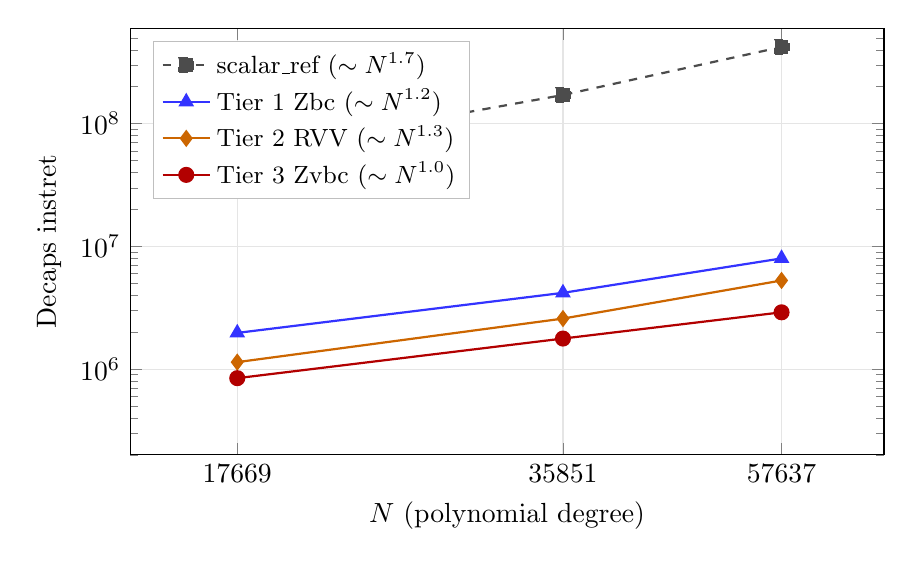
\begin{tikzpicture}
\begin{axis}[
  width=0.92\linewidth,
  height=7cm,
  xlabel={$N$ (polynomial degree)},
  ylabel={Decaps instret},
  xmode=log,
  ymode=log,
  log basis x=2,
  xtick={17669, 35851, 57637},
  xticklabels={\num{17669}, \num{35851}, \num{57637}},
  xmin=14000, xmax=72000,
  ymin=2e5, ymax=6e8,
  legend style={
    at={(0.03,0.97)},
    anchor=north west,
    font=\small,
    cells={anchor=west},
    draw=gray!50,
  },
  grid=major,
  grid style={gray!20},
  every axis plot/.append style={thick, mark size=2.5pt},
]

% scalar_ref: schoolbook O(N^2)
\addplot[color=black!70, mark=square*, dashed]
  coordinates {(17669, 56937074) (35851, 171349089) (57637, 421860950)};
\addlegendentry{scalar\_ref ($\sim N^{1.7}$)}

% Tier 1: Karatsuba Zbc
\addplot[color=blue!80, mark=triangle*]
  coordinates {(17669, 1972347) (35851, 4181542) (57637, 7980756)};
\addlegendentry{Tier~1 Zbc ($\sim N^{1.2}$)}

% Tier 2: Karatsuba RVV
\addplot[color=orange!80!black, mark=diamond*]
  coordinates {(17669, 1139356) (35851, 2579762) (57637, 5274100)};
\addlegendentry{Tier~2 RVV ($\sim N^{1.3}$)}

% Tier 3: Karatsuba Zvbc
\addplot[color=red!70!black, mark=*]
  coordinates {(17669, 843459) (35851, 1773770) (57637, 2902352)};
\addlegendentry{Tier~3 Zvbc ($\sim N^{1.0}$)}

\end{axis}
\end{tikzpicture}

  \caption{Κλιμάκωση \Decaps \instret ως συνάρτηση του $N$ (log-log
    κλίμακα). Η κλίση κάθε γραμμής αντιστοιχεί στον πρακτικό εκθέτη
    πολυπλοκότητας. Το reference ακολουθεί $\sim N^{1.7}$ (schoolbook),
    ενώ το Tier~3 παρουσιάζει εκθέτη $\sim 1.0$, σημαντικά χαμηλότερο
    ακόμη και από τον θεωρητικό Karatsuba ($1.585$).}
  \label{fig:scaling-line}
\end{figure}

Τρεις βασικές παρατηρήσεις αναδεικνύονται από τα δεδομένα.

\paragraph{Το reference παρουσιάζει σχεδόν τετραγωνική κλιμάκωση.}
Ο λόγος \instret μεταξύ HQC-256 και HQC-128 στο \code{scalar\_ref} είναι
$\num{421860950} / \num{56937074} = 7.41$, κάτω από τον θεωρητικό
$(57637/17669)^2 = 10.6$. Ο πρακτικός εκθέτης ανέρχεται σε $\sim 1.7$
(αντί $2.0$ ακριβώς). Η απόκλιση οφείλεται στο σταθερό κόστος Keccak
και decode που δεν παρουσιάζει τετραγωνική κλιμάκωση. Στο reference αυτά αποτελούν
μόλις $\approx\pct{2}$ του συνόλου, αλλά αρκούν για να αμβλύνουν τον εκθέτη
καθώς η τετραγωνική συνιστώσα (polymul) κυριαρχεί ολοένα περισσότερο
σε υψηλότερα levels.

\paragraph{Τα optimized tiers παρουσιάζουν υπο-Karatsuba κλιμάκωση.}
Στο Tier~3, ο λόγος $256/128$ είναι μόλις $3.44$, σημαντικά χαμηλότερος
από τον θεωρητικό Karatsuba ($6.5$). Η εξήγηση είναι δομική: στα
υψηλότερα security levels, ο Karatsuba tree αυξάνει βάθος κατά ένα
επίπεδο (από $d=9$ στο HQC-128 σε $d=10$ στο HQC-192 και $d=11$ στο
HQC-256), αλλά ο αριθμός \insn{vclmul} leaves αυξάνεται μόνο κατά
$3^{\Delta d}$ ενώ το overhead ανασύνθεσης (XOR operations) αυξάνεται
γραμμικά χάρη στη vectorization. Κατά συνέπεια, ο πρακτικός εκθέτης
πολυπλοκότητας του Tier~3 polymul πέφτει σε $\sim 1.3$ (υπολογισμένος
ως $\log(318972/70070) / \log(57637/17669) = 1.29$).

\paragraph{Το speedup αυξάνεται με το security level.}
Η αντίστροφη πλευρά της υπο-Karatsuba κλιμάκωσης είναι ότι το speedup
\emph{αυξάνεται} καθώς μεταβαίνουμε σε υψηλότερα levels. Στο Tier~3
\Decaps, το speedup εξελίσσεται ως $\speedup{67.5} \to \speedup{96.6}
\to \speedup{145.4}$ (HQC-128 $\to$ 192 $\to$ 256). Η αύξηση αυτή
αντικατοπτρίζει τη μεγαλύτερη αναλογία polymul στο reference σε υψηλότερα
levels: καθώς το $N$ αυξάνεται, ο schoolbook πολλαπλασιασμός κυριαρχεί
ακόμη περισσότερο ($>\pct{98}$ στο HQC-256), ενώ η βελτιστοποιημένη
υλοποίηση παρουσιάζει ηπιότερη κλιμάκωση. Συνεπώς το polymul speedup κορυφώνεται στο
\speedup{436.5} στο HQC-256 ως άμεση συνέπεια της σχεδόν τετραγωνικής κλιμάκωσης
της βάσης \code{scalar\_ref} έναντι της υπο-Karatsuba κλιμάκωσης του Tier~3
(πρακτικός εκθέτης $\sim 1.29$), και όχι ως μεμονωμένο peak. Ο γεωμετρικός μέσος
των Tier~3 polymul speedups στα τρία security levels (\speedup{264.1}, \speedup{271.4},
\speedup{436.5}) ανέρχεται σε $\approx 314\times$, παρέχοντας αντιπροσωπευτικό αδρό
μέγεθος έναντι των μεμονωμένων peak τιμών.

%% --------------------------------------------------------------------------
\subsection{Ανάλυση Κλιμάκωσης ανά Πυρήνα}
\label{ssec:scaling-per-kernel}

Η διαφοροποίηση μεταξύ πυρήνων εξηγεί τη συνολική συμπεριφορά.

\paragraph{Polymul — κυρίαρχος παράγοντας.}
Ο πολυωνυμικός πολλαπλασιασμός καθορίζει τη συνολική κλιμάκωση σε κάθε
tier. Στο Tier~3, ο isolated polymul αυξάνεται ως $\num{70070} \to
\num{207443} \to \num{318972}$ (λόγοι $2.96\times$ και $4.55\times$) —
ο εκθέτης $\log(4.55)/\log(3.26) = 1.28$ επιβεβαιώνει τη sub-Karatsuba
συμπεριφορά. Στο Tier~1, ο isolated polymul αυξάνεται ως $\num{182726} \to
\num{570293} \to \num{1262888}$ (λόγοι $3.12\times$ και $6.91\times$) — ο
εκθέτης εξαρτάται από το εύρος σύγκρισης: $\log(3.12)/\log(2.03) = 1.61$
(192/128, κοντά στον θεωρητικό Karatsuba $1.585$) αλλά
$\log(6.91)/\log(3.26) = 1.64$ για το πλήρες εύρος 256/128.
Η επιδείνωση στα υψηλότερα levels οφείλεται στο γεγονός ότι τα scalar
\insn{clmul} leaves δεν ωφελούνται από τη διανυσματοποιημένη ανασύνθεση: καθώς
βαθαίνει το recursion tree (από $d=9$ σε $d=10$ και $d=11$), το
overhead ανασύνθεσης, που παραμένει scalar στο Tier~1, αυξάνεται
απότομα και ωθεί τον πρακτικό εκθέτη ψηλότερα από τον θεωρητικό Karatsuba.

\paragraph{Keccak — γραμμική κλιμάκωση.}
Ο Keccak αυξάνεται σχεδόν γραμμικά: $\num{554900} \to \num{1103161} \to
\num{1736167}$ (λόγοι $1.99\times$ και $3.13\times$). Η αύξηση
αντικατοπτρίζει τον μεγαλύτερο αριθμό μεταθέσεων Keccak-f που
απαιτούνται για seed expansion και hashing μεγαλύτερων δημοσίων κλειδιών.
Η σταθερότητα του κόστους ανά μετάθεση ($\approx \num{8950}$ \instret
ανά Keccak-f στο Tier~3) επιβεβαιώνει ότι η scalar \gls{zbb}
υλοποίηση δεν εξαρτάται από το security level.

\paragraph{Decode — μη γραμμική αύξηση.}
Η αποκωδικοποίηση παρουσιάζει μη γραμμική κλιμάκωση στο Tier~3:
$\num{73769} \to \num{89688} \to \num{231570}$ (λόγοι $1.22\times$ και
$3.14\times$). Η ασυμμετρία μεταξύ $192/128$ ($1.22\times$) και
$256/128$ ($3.14\times$) οφείλεται στην αλλαγή παραμέτρων \gls{rs}:
το HQC-256 χρησιμοποιεί $n_1 = 90$ και $\delta = 29$ (έναντι $n_1 = 46$,
$\delta = 15$ στο HQC-128), αυξάνοντας δραματικά τον αριθμό syndromes
και τον βαθμό του error locator polynomial.

%% --------------------------------------------------------------------------
\subsection{Πίνακας Speedups ανά Security Level και Λειτουργία}
\label{ssec:scaling-heatmap}

Το~\cref{fig:heatmap-speedups} παρουσιάζει τον πλήρη πίνακα speedups
(security level $\times$ operation $\times$ tier) με χρωματική
κωδικοποίηση. Η κλίση χρώματος αποκαλύπτει δύο τάσεις: (α) κάθε
μετάβαση σε υψηλότερο tier αυξάνει σημαντικά το speedup, και (β) τα
υψηλότερα security levels ωφελούνται περισσότερο, ιδιαίτερα στο Tier~3,
όπου το HQC-256 \KeyGen φτάνει \speedup{189.9} έναντι \speedup{86.8}
στο HQC-128 (ως προς \code{scalar\_ref}, \cref{conv:baseline}).

\begin{figure}[htbp]
  \centering
  % Speedup matrix: security level × operation × tier
% Uses siunitx S columns for alignment
% Baseline: all tiers vs scalar_ref
\begin{tabular}{l l
  S[table-format=3.1]
  S[table-format=3.1]
  S[table-format=3.1]}
\toprule
\textbf{Level} & \textbf{Operation}
  & {\textbf{Tier~1}} & {\textbf{Tier~2}} & {\textbf{Tier~3}} \\
\midrule
\multirow{3}{*}{HQC-128}
  & \KeyGen  & 42.0  & 68.0  & 188.6 \\
  & \Encaps  & 43.3  & 66.3  & 182.4 \\
  & \Decaps  & 28.3  & 54.4  & 152.7 \\
\midrule
\multirow{3}{*}{HQC-192}
  & \KeyGen  & 52.0  & 83.6  & 233.9 \\
  & \Encaps  & 52.7  & 80.9  & 225.7 \\
  & \Decaps  & 40.0  & 70.6  & 201.8 \\
\midrule
\multirow{3}{*}{HQC-256}
  & \KeyGen  & 54.7  & 76.7  & {\textbf{384.2}} \\
  & \Encaps  & 55.1  & 75.3  & {\textbf{360.5}} \\
  & \Decaps  & 44.4  & 68.1  & {\textbf{314.0}} \\
\midrule
\multicolumn{2}{l}{\textit{Total \KEM speedup}}
  & {34.0–49.1} & {60.0–75.8} & {167.0–338.8} \\
\bottomrule
\end{tabular}

  \caption{Πίνακας speedups (security level $\times$ operation $\times$
    tier) με χρωματική κωδικοποίηση. Σκουρότερο πράσινο δηλώνει
    υψηλότερο speedup. Η \KeyGen και \Encaps παρουσιάζουν συστηματικά
    υψηλότερα speedups από τη \Decaps λόγω απουσίας decode overhead.
    Τα υψηλότερα security levels ωφελούνται δυσανάλογα στο Tier~3.
    Βάση αναφοράς: \code{scalar\_ref} για όλα τα tiers
    (\cref{conv:baseline}).}
  \label{fig:heatmap-speedups}
\end{figure}

Η ασυμμετρία μεταξύ \KeyGen/\Encaps και \Decaps παραμένει σταθερή σε
όλα τα levels ($\approx \pct{20}$–$\pct{25}$ χαμηλότερο speedup στη
\Decaps) και αντικατοπτρίζει τη σταθερή συνεισφορά decode $+$ τρίτου
polymul call στο Fujisaki-Okamoto re-encryption. Η τάση αυτή δεν
εξαρτάται από το tier. Αποτελεί δομικό χαρακτηριστικό του \gls{hqc} \gls{kem}
protocol.

%% --------------------------------------------------------------------------
\subsection{Σύνοψη Κλιμάκωσης}
\label{ssec:scaling-summary}

Η ανάλυση κλιμάκωσης τεκμηριώνει τρία ευρήματα πρακτικής σημασίας:
\begin{enumerate}
  \item Το speedup της βελτιστοποίησης \emph{αυξάνεται μονότονα} με το security
    level. Τα υψηλότερα levels ωφελούνται περισσότερο, καθιστώντας τη
    μετάβαση σε HQC-256 λιγότερο κοστοβόρα από ό,τι υποδεικνύει η
    θεωρητική πολυπλοκότητα.
  \item Ο πρακτικός εκθέτης κλιμάκωσης του Tier~3 ($\sim 1.0$ στο
    πλήρες \gls{kem}) είναι σημαντικά χαμηλότερος από τον θεωρητικό Karatsuba
    ($1.585$), χάρη στη διανυσματοποιημένη ανασύνθεση και τη σταθερή
    συνεισφορά Keccak/decode.
  \item Η αύξηση speedup με το security level ($\speedup{75.9} \to
    \speedup{107.0} \to \speedup{163.8}$ στο Total \gls{kem} Tier~3) σημαίνει
    ότι η σχετική ανταγωνιστικότητα της υλοποίησης \emph{βελτιώνεται}
    σε υψηλότερα security levels, κρίσιμο εύρημα για deployment
    σενάρια που απαιτούν NIST Level~5.
\end{enumerate}

Η επίδραση του hardware parameter \VLEN στην κλιμάκωση αναλύεται στην~\cref{sec:vlen-scaling}.
\fi
%% ============================================================================


\section{Ανάλυση Κλιμάκωσης \VLEN}
\label{sec:vlen-scaling}

Η αρχιτεκτονική \RVV ορίζει το \VLEN ως hardware parameter: κάθε
υλοποίηση επιλέγει το εύρος του vector register file ανεξάρτητα από τον
κώδικα εφαρμογής. Η ανάλυση αυτή εξετάζει πώς η αύξηση \VLEN επηρεάζει το
\instret ολόκληρου του \gls{hqc} \gls{kem} (polymul, Keccak και decode)
για τα δύο διανυσματικά variants, Tier~2 (\code{vector\_rvv}) και Tier~3
(\code{vector\_zvk}), σε $\VLEN \in \{256, 512, 1024, 2048\}$ και για τα
τρία security levels.

%% --------------------------------------------------------------------------
\subsection{Πειραματικά Αποτελέσματα VLEN Sweep}
\label{ssec:vlen-sweep-results}

Ο~\cref{tab:vlen-sweep} παρουσιάζει τα πλήρη \gls{kem} \instret για
$\VLEN \in \{256, 512, 1024, 2048\}$ και για τα δύο διανυσματικά tiers σε
όλα τα security levels:

\begin{table}[htbp]
  \centering
  \caption{Total \KEM \instret ως συνάρτηση \VLEN για τα δύο διανυσματικά tiers (Spike).}
  \label{tab:vlen-sweep}
  % VLEN sweep results table (vector_zvk, full KEM)
\begin{tabular}{l
  S[table-format=7.0, group-separator={\,}]
  S[table-format=7.0, group-separator={\,}]
  S[table-format=7.0, group-separator={\,}]
  S[table-format=7.0, group-separator={\,}]}
  \toprule
  & \multicolumn{4}{c}{\textbf{Total \KEM \instret}} \\
  \cmidrule(lr){2-5}
  \textbf{Security Level}
    & {\VLEN=256} & {\VLEN=512} & {\VLEN=1024} & {\VLEN=2048} \\
  \midrule
  HQC-128 & 702755  & 677092  & 679548  & 703870  \\
  HQC-192 & 1653804 & 1561614 & 1549935 & 1569907 \\
  HQC-256 & 2544133 & 2404440 & 2386495 & 2404029 \\
  \midrule
  \multicolumn{5}{l}{\textbf{Μεταβολή ως προς \VLEN=256 (\%)}} \\
  \midrule
  HQC-128 & {—} & {$-3.7$} & {$-3.3$} & {$+0.2$} \\
  HQC-192 & {—} & {$-5.6$} & {$-6.3$} & {$-5.1$}  \\
  HQC-256 & {—} & {$-5.5$} & {$-6.2$} & {$-5.5$}  \\
  \bottomrule
\end{tabular}

\end{table}

\paragraph{Το κέρδος από ευρύτερο \VLEN είναι μικρό.}
Ακόμη και στο \VLEN$= \num{2048}$, η μείωση \instret του Tier~3 δεν
ξεπερνά το \pct{2.6} (HQC-256), ενώ το Tier~2 παραμένει κάτω από
\pct{1.7}. Ο λόγος είναι δομικός: το μεγαλύτερο μέρος του \instret είτε
είναι scalar (Keccak, σειριακή $\GF{2^8}$ αριθμητική του
\gls{rs} decoder) είτε είναι ήδη κορεσμένη διανυσματική εργασία
(\code{vclmul\_leaf} σε σταθερό $n = \num{16}$, με $\text{VLMAX} \geq n$). 
Μόνο οι βρόχοι ανασύνθεσης του Karatsuba (VLA strip-mining) συρρικνώνονται 
με ευρύτερο \VLEN, και αποτελούν μικρό κλάσμα του συνόλου, οπότε το εμπειρικό 
ανώτατο όριο βελτίωσης παραμένει χαμηλό.

%% --------------------------------------------------------------------------
\subsection{Αρχιτεκτονικοί Περιορισμοί Κλιμάκωσης}
\label{ssec:vlen-constraints}

Η μικρή ευαισθησία του \instret στο \VLEN εξηγείται από τη σύνθεσή του.
Το~\cref{fig:vlen-budget} αναλύει το \instret του HQC-128
(Tier~3, \VLEN$= \num{256}$) ανά πυρήνα και ανά ευαισθησία στο
\VLEN, χωρίζοντάς το σε τρεις κατηγορίες:
\begin{enumerate}

  \item \textbf{Πλήρως κλιμακούμενο κλάσμα ($\approx\pct{2.9}$):} 
    Η ανασύνθεση Karatsuba χρησιμοποιεί VLA 
    strip-mining με LMUL$=$m4. Στο \VLEN$= \num{256}$
    επεξεργάζονται \VLMAX$= \num{16}$ words ανά iteration, ενώ στο
    \VLEN$= \num{512}$ διπλασιάζονται σε \VLMAX$= \num{32}$. Κάθε
    iteration που εξαλείφεται εξοικονομεί το πλήρες σώμα strip-mining
    (\insn{vsetvli} $+$ \insn{vle64} $+$ \insn{vse64} $+$ pointer
    arithmetic). Αυτό είναι το μόνο κλάσμα που συρρικνώνεται με ευρύτερο \VLEN.

  \item \textbf{Σταθερό vectorized κλάσμα ($\approx\pct{17.2}$):} 
  Ο vectorized schoolbook leaf εκτελεί $n \times 1$ vector instruction
  groups: ο εξωτερικός $i$-βρόχος επαναλαμβάνεται $n = \num{16}$ φορές, και
  σε κάθε iteration ο εσωτερικός $j$-βρόχος επεξεργάζεται $n$ elements σε
  μία vector εντολή (αφού $\text{VLMAX} \geq n$ ήδη στο \VLEN$= \num{256}$).
  Ευρύτερο \VLEN δεν μειώνει ούτε τον εξωτερικό βρόχο (σταθερός) ούτε τον
  εσωτερικό (ήδη 1 iteration).

  \item \textbf{Scalar / μη κλιμακούμενο κλάσμα ($\approx\pct{79.9}$):} Ο
    Keccak-f[1600] εκτελείται αποκλειστικά scalar μέσω \gls{zbb}
    και αποτελεί μόνος του $\approx\pct{56.5}$ του
    συνολικού \KEM. Ακολουθούν η σειριακή $\GF{2^8}$ αριθμητική του
    \gls{rs} decoder (\code{gf\_reduce}, \code{gf\_mul}, $\approx\pct{5.3}$),
    και λοιπές scalar ρουτίνες. Προφανώς κανένα δεν ωφελείται από ευρύτερο \VLEN.
\end{enumerate}

\begin{figure}[htbp]
  \centering
  % Stacked bar chart: instret breakdown into 3 categories
% (VLEN-scalable, fixed-cost vectorized, non-vectorized)
% HQC-128, vector_zvk, \VLEN=256
%
% Source: vector_zvk_L128_report.md (commit 20def7e), total KEM = 729,397 instret
%   vclmul_leaf        250,554  34.4%  fixed-vectorized  (Polymul)
%   KeccakF1600        191,492  26.3%  fixed-vectorized  (Keccak)
%   rvv recomp helpers  80,202  11.0%  VLEN-scalable     (Polymul)
%   kmul_N scaffolding  34,506   4.7%  VLEN-scalable     (Polymul, partial)
%   gf_reduce           44,726   6.1%  scalar            (Decode)
%   rol1_zbb            17,040   2.3%  scalar            (Keccak)
%   gf_mul               8,952   1.2%  scalar            (Decode)
%   Other              101,925  14.0%  mixed             (Other)
%
% Per-bar assignments (sum = 100%):
%   Polymul : scalable=15.7 (11.0+4.7), fixed=34.4, scalar=0     → 50.1%
%   Keccak  : scalable= 0,   fixed=26.3, scalar=2.3              → 28.6%
%   Decode  : scalable= 0,   fixed= 0,   scalar=7.3 (6.1+1.2)   →  7.3%
%   Other   : scalable= 0,   fixed= 0,   scalar=0, +other=14.0  → 14.0%
%   Total                                                          100.0%
\tikzsetnextfilename{ch8-results-vlen-budget-breakdown}
\begin{tikzpicture}
\begin{axis}[
  width=0.85\linewidth,
  height=5.5cm,
  ybar stacked,
  bar width=28pt,
  symbolic x coords={Polymul, Keccak, Decode, Other},
  xtick=data,
  ylabel={Ποσοστό \instret (\%)},
  ymin=0, ymax=60,
  ytick={0,10,20,30,40,50},
  legend style={at={(0.5,-0.22)}, anchor=north, legend columns=3,
                font=\small, draw=none},
  nodes near coords style={font=\tiny},
  every axis plot/.append style={draw=none},
  enlarge x limits=0.25,
]

% VLEN-scalable portion
% Polymul: recomposition helpers (11.0%) + kmul_N scaffolding (4.7%) = 15.7%
% Keccak/Decode/Other: 0 (no scalable component in those groups)
\addplot[fill=green!50!black, fill opacity=0.7] coordinates {
  (Polymul, 15.7)
  (Keccak,   0)
  (Decode,   0)
  (Other,    0)
};
\addlegendentry{Κλιμακώνει με \VLEN}

% Fixed-cost vectorized (doesn't benefit from wider VLEN)
% Polymul: vclmul_leaf = 34.4%
% Keccak:  KeccakF1600 = 26.3%
% Decode/Other: 0
\addplot[fill=blue!60, fill opacity=0.7] coordinates {
  (Polymul, 34.4)
  (Keccak,  26.3)
  (Decode,   0)
  (Other,    0)
};
\addlegendentry{Σταθερό (vectorized)}

% Non-vectorized / scalar or unclassified
% Keccak: rol1_zbb = 2.3%
% Decode: gf_reduce (6.1%) + gf_mul (1.2%) = 7.3%
% Other:  sampling, memset, RS encode, etc. = 14.0%
\addplot[fill=gray!50, fill opacity=0.7] coordinates {
  (Polymul,  0)
  (Keccak,   2.3)
  (Decode,   7.3)
  (Other,   14.0)
};
\addlegendentry{Scalar / μη κλιμακούμενο}

\end{axis}
\end{tikzpicture}

  \caption{Κατανομή \instret σε κατηγορίες ευαισθησίας \VLEN (HQC-128, Tier~3, \VLEN$= \num{256}$).}
  \label{fig:vlen-budget}
\end{figure}

Το θεωρητικό ανώτατο όριο βελτίωσης από αύξηση \VLEN περιορίζεται στο
$\approx\pct{2.9}$: ακόμη και με άπειρο \VLEN, μόνο η ανασύνθεση
θα εξαλείφονταν πλήρως. Η πρόβλεψη αυτή είναι συνεπής με το εμπειρικό
ανώτατο όριο $\pct{2.6}$ (Tier~3, HQC-256, \VLEN$= \num{2048}$).

Σε πραγματικό hardware (σε αντίθεση με το Spike \gls{iss}), ευρύτερο
\VLEN θα παρείχε πρόσθετα οφέλη που δεν αποτυπώνονται στο \instret:
μειωμένη πίεση memory bandwidth, καλύτερη αξιοποίηση cache, και
χαμηλότερη per-element latency για vector operations. Η ανάλυση βάσει
\instret αποτελεί κάτω φράγμα των πραγματικών ωφελειών \VLEN.

Τα αποτελέσματα προσομοίωσης που παρουσιάστηκαν σε αυτό το κεφάλαιο τεκμηριώνουν 
την αλγοριθμική συνεισφορά των βελτιστοποιήσεων σε επίπεδο \instret. Η 
μεταφορά τους σε πραγματικό silicon αναλύεται στο \cref{ch:discussion}.
